\documentclass[12pt]{article}

\usepackage{fullpage}	
\usepackage{amsmath,amsthm,amssymb}
\usepackage{graphicx}	
\usepackage[square, authoryear, sort, comma, numbers]{natbib}	
\usepackage{setspace}
\usepackage[T1]{fontenc}
\usepackage{titling}
\usepackage{enumerate}
\usepackage{float}
\usepackage{titlesec}
\usepackage{makeidx}
\usepackage{wrapfig}

\titleformat{\section}
  {\normalfont\fontsize{14}{15}\bfseries}{\thesection}{1em}{}

\titleformat{\subsection}
  {\normalfont\fontsize{14}{15}\bfseries}{\thesubsection}{1em}{}

\setlength{\droptitle}{-5em}   
\newcommand*{\TitleFont}{%
      \usefont{\encodingdefault}{\rmdefault}{n}{b}%
      \fontsize{14}{16}%
      \selectfont}

\begin{document}

\title{\TitleFont \textbf{Connect N:\\ A Reinforcement Learning Approach}}
\author{\TitleFont Lucy Cheng, Angela Fan, Andre Nguyen}
\date{}
\maketitle

\vspace{-1.5cm}

\section{Problem Description}

The problem we chose to work on is that of the classic children's game, Connect-4, but extrapolated to be "Connect-N", where players strive to create streaks of length N with their tokens, while stopping their opponent from creating N-length streaks.

\section{Simulator and Driver Function Descriptions}

The \textbf{simulator} takes two inputs:
\begin{enumerate}
\item \textbf{n}, the number of tokens that must be connected by a player to win
\item \textbf{grid\_size}, the height of the square board that will be created by the simulator
\end{enumerate}

The simulator initializes a nested NumPy array of zeroes, where each nested array is a row of the board. Zero represents an empty state. Players 1 and -1 can tell the simulator to make a move by calling the simulator's move method. The board state then adds a 1 or -1 (depending on the player) in the correct spot. When the move method is called, the simulator automatically checks if a player has won. 

The move function returns:

\begin{enumerate}
\item 1 if the current player making a move has won
\item -1 if the current player making a move is trying to make an illegal move (for example: column does not exist, column is already full)
\item 0 otherwise
\end{enumerate}

and a reward:
\begin{enumerate}
\item 50 if the current player making a move has won
\item 0 otherwise
\end{enumerate}

The simulator has a number of helper methods as well:
\begin{enumerate}
\item \textbf{simulate\_move}, which tests to see if a move is valid and returns 1 if not valid
\item \textbf{turn}, which returns whose turn it is 
\item \textbf{next\_possible\_moves}, which returns an array of all possible columns available for a next move (i.e. eliminates columns that are full)
\item \textbf{all\_tokens\_placed}, which returns the location as a (column, row) tuple of all of the tokens that have been placed					
\item \textbf{is\_empty}- takes in a location and returns True if the location is empty and False otherwise
\item \textbf{streak} functions that check if a given player has a horizontal, vertical, or diagonal streak going
\item \textbf{print\_grid}, which prints the current board state
\end{enumerate}

We have written a separate function, called \textbf{play\_game}, that serves as a driver function to run the Connect N game (diagrammed in \textbf{Figure 1}).  The driver function takes as input two learners, and uses the Connect N simulator to create a game. The game asks each learner for an action and takes the specified moves. If neither player has won, it continues the game by passing reward and the new board state back to the learners.

\begin{figure}
\centering
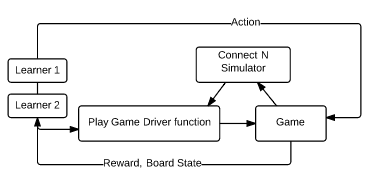
\includegraphics[scale=.7]{game_process.png}
\caption{Play Game Driver Function}
\end{figure}

\section{State and Action Spaces}

Possible \textbf{actions} are integers representing the numerical column number that a player wishes to put their token into.

The \textbf{states} are boards, represented as NumPy arrays. The board is initialized to be full of zeros, which represent empty token spots. Player 1's tokens replace the 0 with 1, and player -1's tokens replace the 0 with -1. 

\section{Approaches}

\begin{figure}
\centering
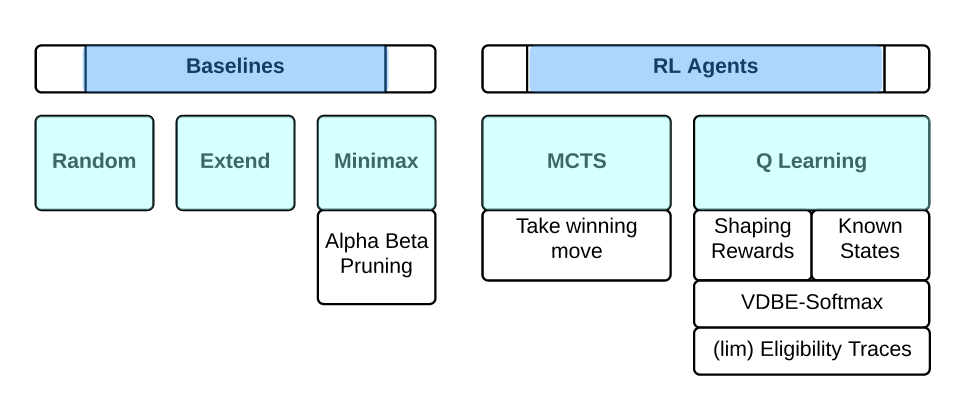
\includegraphics[scale=.5]{learners.png}
\caption{Implemented Baselines and Learners, with Extensions}
\end{figure}

\subsubsection{Baselines} 

We implemented three baselines:
\begin{enumerate}
\item \textbf{Random action}, where the agent randomly chooses a column to put its token into at each time step
\item \textbf{Extend}, where the agent attempts to extend its largest current streak (horizontally, vertically, or diagonally), breaking ties between streaks randomly.
\item \textbf{Minimax}--- We implemented the Artificial Intelligence algorithm Minimax, which conceptualizes the Connect-N game as a tree of possible future game states. The current state of the game is the root node of the tree, and each of the children represent possible states resulting from a move that can be made from the current game state. The leaves are the final states of the game, or states where no further moves can be made because one player has one or lost. In traditional Minimax, leaves have a value of either positive infinity (win), negative infinity (lose), or 0 (tie), but such an algorithm forces Minimax to continue evaluating future board states until it reaches a win or a lose. However, this is often computationally infeasible as there are so many possible states in the game. Instead, we implement a \textbf{static evaluation} form of Minimax that takes a \textbf{depth} parameter that governs how far down the tree the algorithm should explore. We generate node values in Minimax according to this heuristic:

\begin{itemize}

\item Each streak contributes a value of $x * 2^x/2$, where $x$ is the length of the streak, except when $x = n$, where the streak contributes a value of $2000000$.
\item Each opponent streak contributes a value $-(x *  2^x) / 6$, where x is the length of the streak, except when $x = n$, where the streak contributes a value of $-1000000$.
\end{itemize}
The motivation for these values was that longer streaks are closer to the goal state, and therefore should have much higher value. We chose $2^{x-1}$ at first, but found the agent prioritizing creating multiple streaks of length $x$ instead of creating a streak of $x-1$, so we increased the difference in value between streaks even more. At first, we did not have negative values for opponent streaks, which resulted in very boring games between Minimax agents, since there was little interaction between the agents, and the first player always won. The negative value for opponent streaks was added to incentivize agents to try to block the progress of their opponent. We divided by an extra factor of 3 so agents would still prioritize extending their own streak over blocking an opponent streak of the same length. The values for $x=n$ are chosen to represent $\infty$ since they represent winning or losing the game.

We also explore an extension to Minimax, called \textbf{alpha-beta pruning}, motivated by the idea that often Minimax explores more branches than is required. For example, if it needs to expand down to depth 3, but is currently at depth 2, it will continue expanding all branches to depth 3 even if one branch clearly would lead to a loss. In alpha-beta pruned Minimax, the tree is pruned to only continue investigating good paths. The algorithm controls the range of values the tree should continue searching down, and we initialize this range to $\pm 1000$ for generality.

\end{enumerate}

\subsubsection{Q Learning}

The first reinforcement learning approach we looked at was Q Learning, an off-policy TD control algorithm that we investigated in Practical 1. The straightforward version of Q Learning we implemented in Practical 1 did not seem like it could have any chance of performing as well as an AI algorithm such as Minimax, so we additionally implemented a number of extensions to Q Learning.

\begin{enumerate}
\item We replaced $\epsilon$-greedy with the \textbf{VDBE-Softmax} policy described in [Tokic, 2011]. When evaluated on the Gridworld, VDBE-Softmax outperformed $\epsilon$-greedy in cumulative reward substantially, so we thought it could potentially do better in Connect-N as well.
\item We implemented \textbf{eligibility traces}, as described in the Sutton and Barto textbook and as we covered in class discussions, as it can help the learner learn more efficiently. Unfortunately, the complete eligibility traces algorithm iterates over all states and actions, which was computationally infeasible in this game, as the states represent all possible versions of the Connect N board state. Instead, we implement a limited version of eligibility traces, where the algorithm updates $Q(s, a)$ and $e(s, a)$ for each board state it currently knows and all board states that can be reached by taking one action from the current board state.
\item We implemented a version of \textbf{known states}, where some classes of board states are given a known value. Since our Q Learner only stores states as we reach them, due to space constraints, our implementation of known states does not initialize values for states. Instead, at each board state, we check for certain conditions, and populate the value table then if the conditions are satisfied. First, for each possible action, we checked if the action would create a streak of length greater than or equal to $n-1$. If so, we give it a value of 15. For reference, a winning action has value 25. Second, we checked if the action would directly prevent an opponent win, and gave the action value 20, which guarantees our learner would prevent enemy wins. The implementation of known states for Q Learning was inspired and based on the heuristics for Minimax, since the idea of both is to estimate the value of a state.
\end{enumerate}

\begin{wrapfigure}{l}{5cm}
	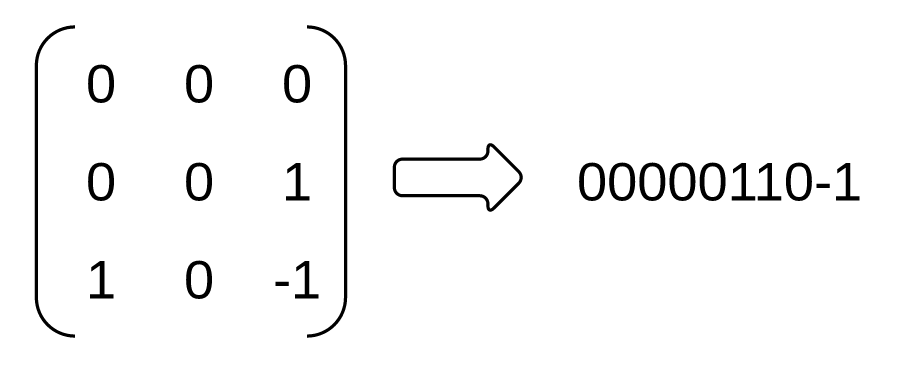
\includegraphics[scale=.16]{transform}
\end{wrapfigure}

The Q learner continues to keep an action value table (as in Practical 1), with a slightly different data structure. The Q learner takes the board state and hashes it into a string, where 0 represents an empty spot and 1 and -1 represent self and opponent tokens. It then adds the string board state as a key into a dictionary. For computational reasons, instead of adding all of the possible board states to the dictionary, the dictionary only ever holds board states that it has seen. 

To pre-train the Q learner, we pass the board state between different games, allowing the Q learner to have a better, more competitive knowledge of what actions are good or bad.

\subsubsection{Monte Carlo Tree Search- andre} 


\section{detailed description of your results/comparisons- everyone- wait for results}

\begin{table}[h]
\begin{tabular}{llllllllllll}
Player 1 (row) / Player 2 (col) & Random                                                                                                                        & Extend            & MCTS                              & Minimax depth-2                             & Minimax depth-2 'ab' & Minimax depth-4                                              & Minimax depth-4 'ab' & Minimax depth-5   & Minimax depth-5 'ab' & Q-Learning                                & Q-Learning w/ Known States \\

Random                          & 0.5607 / 0.0002 / 0.4391                                                                                                      & 0.04 / 0.0 / 0.96 & 0.2 / 0.0 / 0.8                   & 0.13 / 0.0 / 0.87                           & 0.65 / 0.0 / 0.35    & \begin{tabular}[c]{@{}l@{}}0.01 / \\ 0.0 / 0.99\end{tabular} & 0.02 / 0.0 / 0.98    & 0.03 / 0.0 / 0.97 & 0.0 / 0.0 / 1.0      &                                           &                            \\
Extend                          &                                                                                                                               &                   &                                   & 0.0 / 0.0 / 1.0                             &                      &                                                              &                      &                   &                      &                                           &                            \\
MCTS                            &                                                                                                                               &                   &                                   &                                             &                      &                                                              &                      &                   &                      &                                           &                            \\
Minimax depth-2                 &                                                                                                                               &                   &                                   & 0.0 / 0.0 / 1.0 (0.0 / 0.0 / 1.0 w/ forced) &                      &                                                              &                      &                   &                      &                                           &                            \\
Minimax depth-2 'ab'            &                                                                                                                               &                   &                                   &                                             &                      &                                                              &                      &                   &                      &                                           &                            \\
Minimax depth-4                 &                                                                                                                               &                   &                                   &                                             &                      & 0.0 / 0.0 / 1.0 (1.0 / 0.0 / 0.0)                            &                      &                   &                      &                                           &                            \\
Minimax depth-4 'ab'            &                                                                                                                               &                   &                                   &                                             &                      &                                                              &                      &                   &                      &                                           &                            \\
Minimax depth-5                 &                                                                                                                               &                   &                                   &                                             &                      &                                                              &                      &                   &                      &                                           &                            \\
Minimax depth-5 'ab'            &                                                                                                                               &                   &                                   &                                             &                      &                                                              &                      &                   &                      &                                           &                            \\
Q-Learning                      & \begin{tabular}[c]{@{}l@{}}0.7604 / 0.1118 / 0.1278 (trained 10000) -\\ 0.7493 / 0.1209 / 0.1298 (trained 22000)\end{tabular} &                   & 0.75 / 0.05 / 0.2 (trained 32000) & 0.139 / 0.351 / 0.51 (trained 20000)        &                      & 0.0 / 0.4 / 0.6 (trained 21000)                              &                      &                   &                      & 0.0876 / 0.8439 / 0.0685 (both untrained) &                            \\
Q-Learning w/ Known States      & 0.7502 / 0.1192 / 0.1306 (trained 10000) - 0.7503 / 0.1201 / 0.1296 (trained 22000)                                           &                   &                                   & 0.149 / 0.334 / 0.517 (trained 20000)       &                      & 0.001 / 0.487 / 0.512 (trained 21000)                        &                      &                   &                      & 0.0905 / 0.8438 / 0.0657 (both untrained) &                           
\end{tabular}
\end{table}


\section{thorough description of why you got the results you did, a few pages- everyone- wait for results}


\section{Future Work}

Interesting research questions for the future could include:

\begin{enumerate}
\item Exploring extensions to MCTS, such as a better default policy (perhaps estimation of a value for each board state, and selecting the action that leads to the board state with highest value)
\item Exploring large N, where computational complexity of solving MCTS and Minimax could potentially allow Q learning to perform competitively (as MCTS iteration number would be low and Minimax depth parameter would be low)
\item Adding stochasticity to the board, such as dropping the bottom row with some probability or having a probability of taking the wrong action
\item Coding the board state as a POMDP, with information such as the number of tokens in a row, but not knowing exactly where the tokens are 
\end{enumerate}



\end{document}







